\chapter{Svolgimento dello \textit{stage}} 
\label{cap:descrizione-stage}

\section{Flusso di lavoro}
\subsection{Pianificazione delle attività}
In accordo agli obiettivi descritti in \ref{sec:obiettiviStage}, ho redatto, insieme al \textit{tutor} aziendale, una pianficazione settimanale delle attività da svolgere.
Nella tabella \ref{tab:prevAttività} presento la pianificazione di tali attività.

\renewcommand{\arraystretch}{2}
\begin{longtable}{|p{3cm}|p{9cm}|} 
    \hline
    \rowcolor{tableheader}\textbf{Periodo} & \textbf{Descrizione attività} \\
    \hline
    \endfirsthead

    \rowcolor{tableheader}\textbf{Periodo} & \textbf{Descrizione attività} \\
    \hline
    \endhead

    \hline
    \endfoot

    \hline
    \endlastfoot
    \rowcolor{tableevenrow} Prima settimana & \begin{tabular}[t]{@{}p{9cm}@{}}
        - Studio ed apprendimento delle tecnologie di sviluppo \\
        - Definizione delle \textit{user stories} \\
    \end{tabular} \\
    \hline
    \hline
    \rowcolor{tableoddrow} Seconda settimana &  \begin{tabular}[t]{@{}p{9cm}@{}}
        - Creazione \textit{ticket} di \textit{mock} \\
        - Caricamento dei \textit{ticket} all'interno dell'\gls{its} Jira
    \end{tabular} \\
    \hline
    \rowcolor{tableevenrow} Terza settimana & \begin{tabular}[t]{@{}p{9cm}@{}}
        - Reperire i ticket completati da Jira\\
        - Salvataggio \textit{ticket} su \textit{database} MongoDB \\
        - Aggiornamento costante del \textit{database}\\
    \end{tabular} \\
    \hline
    \rowcolor{tableoddrow} Quarta settimana & \begin{tabular}[t]{@{}p{9cm}@{}}
        - Studio \gls{embedding-g} per \gls{rag-g}\\
        - Tokenizzazione dei \textit{ticket} contenuti nel \textit{database} MongoDB \\
        - Connessione tra AWS Bedrock e MongoDB per \gls{rag-g}\\
    \end{tabular} \\
    \hline
    \rowcolor{tableevenrow} Quinta settimana & \begin{tabular}[t]{@{}p{9cm}@{}}
        - Creazione di domande di \textit{benchmark}\\
        - Confronto tra i diversi \gls{llm}, modelli progettati per generare testo umano\\
    \end{tabular} \\
    \hline
    \rowcolor{tableoddrow} Sesta settimana & \begin{tabular}[t]{@{}p{9cm}@{}}
        - Aggiornamento del \textit{ticket} Jira con la proposta di risoluzione, generata tramite il sistema di IA Generativa\\
        - Sviluppo di un \textit{chatbot} per l'interrogazione sui \textit{ticket} Jira\\
    \end{tabular} \\ 
    \hline
    \rowcolor{tableevenrow} Settima settimana & \begin{tabular}[t]{@{}p{9cm}@{}}
        - Migliorie al sistema di proposte di risoluzione Jira\\
        - Migliorie al \textit{chatbot}, dando all'utente la possibilità di utilizzare \gls{llm} diversi \\
        - Implementare un sistema di autenticazione nel \textit{chatbot} \\
    \end{tabular} \\ 
    \hline
    \rowcolor{tableoddrow} Ottava settimana & \begin{tabular}[t]{@{}p{9cm}@{}}
        - Realizzazione di una presentazione sui progetti sviluppati\\
        - Redazione documento manuale utente \\
        - Redazione documento sull'architettura e sulle scelte progettuali adottate \\
        - Miglioria al \textit{chatbot} per proposte di risoluzione più descrittive \\
    \end{tabular} \\ 
    \hline
    \caption{Pianificazione del progetto di \textit{stage}}
    \label{tab:prevAttività}
\end{longtable}

\subsection{Revisioni di progetto} \label{sec:revisioni}
L'attività di revisione del progetto ritengo essere stata di fondamentale importanza e più utile ai fini formativi dello \textit{stage}.
Nel corso del tirocinio ho avuto modo di sperimentare due tipologie di revisione: il \textit{daily}, un incontro giornaliero con il \textit{tutor} aziendale, e lo \textit{sprint review}, un incontro settimanale con il \textit{tutor} aziendale per valutare quanto avevo svolto durante la settimana e pianificare le attività per la settimana successiva.
L'occorrenza del \textit{daily} è stata purtroppo però limitata a causa di numerosi impegni che il \textit{tutor} aziendale aveva durante la giornata. Sono stati comunque utili, soprattutto all'inizio dello \textit{stage}, per chiarire dubbi su come procedere con le attività e per ricevere feedback immediato su quanto svolto.
Lo \textit{sprint review} invece è stato quello presente con regolarità assoluta, che mi ha permesso di ricevere un feedback più dettagliato su quanto avevo svolto durante la settimana, che mi hanno permesso di correggere eventuali errori e di migliorare la qualità del lavoro svolto.

\subsection{Interazioni con il tutor aziendale}
Come descritto nella sezione \ref{sec:revisioni}, le interazioni con il \textit{tutor} aziendale sono state numerose e di fondamentale importanza per il corretto svolgimento delle attività.
Nelle giornate in cui non era possibile riferirmi direttamente al \textit{tutor} aziendale, mi sono rivolto ad una figura di supporto, che in caso di assenza o indisponibilità del \textit{tutor} aziendale, era predista all'aiuto degli stagisti in caso di problematiche.
\section{Analisi preventiva dei rischi}
I primi giorni di stage sono stati dedicati all'individuazione dei potenziali rischi che avrei potuto incontrare durante lo svolgimento dello \textit{stage}.
Si farà riferimento ai rischi individuati (R) seguendo la seguente notazione: 
\begin{center}
    \textbf{R-[Tipologia]-[Probabilità][Impatto]-[Indice]}
\end{center}
dove:
\begin{itemize}
    \item \textbf{Tipologia}: \\ Natura del rischio: \begin{itemize}
        \item \textbf{T}: Tecnologico
        \item \textbf{O}: Organizzativo
        \item \textbf{P}: Personale
    \end{itemize}
    \item \textbf{Probabilità}: \\ Numero intero positivo che indica la probabilità di occorrenza del rischio: \begin{itemize}
        \item \textbf{1}: Alta
        \item \textbf{2}: Media
        \item \textbf{3}: Bassa
    \end{itemize}
    \item \textbf{Impatto}: \\ Valore alfabetico che indica la probabilità di occorrenza del rischio: \begin{itemize}
        \item \textbf{A}: Alto
        \item \textbf{B}: Medio
        \item \textbf{C}: Basso
    \end{itemize}
    \item \textbf{Indice}: Numero intero positivo incrementale che determina univocamente il rischio relativamente ad una specifica tipologia
\end{itemize}

\renewcommand{\arraystretch}{2}
\begin{longtable}{|p{3cm}|p{4.3cm}|p{4.5cm}|} 
    \hline
    \rowcolor{tableheader}\textbf{Codice} & \textbf{Descrizione} & \textbf{Mitigazione} \\
    \hline
    \endfirsthead

    \rowcolor{tableheader}\textbf{Codice} & \textbf{Descrizione} & \textbf{Mitigazione} \\
    \hline
    \endhead

    \hline
    \endfoot

    \hline
    \endlastfoot

    \rowcolor{tableevenrow} R-T-1A-1 & Complessità del contesto di uso di servizi di IA Generativa & 
    Chiedere supporto al \textit{tutor} aziendale sul corretto utilizzo dei servizi di IA Generativa che verranno utilizzati \\
    \hline
    \rowcolor{tableoddrow} R-T-2B-2 & Complessità del contesto di sviluppo e attività di integrazione con la \textit{suite} Atlassian & 
    \begin{tabular}[t]{@{}p{4.3cm}@{}}
        - Riferimento a documentazione più dettagliata \\
        - Supporto da parte del \textit{tutor} aziendale \\
    \end{tabular} \\
    \hline
    \rowcolor{tableevenrow} R-T-1A-3 & Ridotta conoscenza dei servizi cloud \gls{aws} & 
    \begin{tabular}[t]{@{}p{4.3cm}@{}}
        - Studio approfondito dei servizi \gls{aws} \\
        - Documentazione dettagliata dei servizi \gls{aws} \\
        - Supporto da parte del \textit{tutor} aziendale
    \end{tabular} \\
    \hline
    \rowcolor{tableoddrow} R-P-3C-1 & Assenze per motivi di salute o personali & 
    Avvisare per tempo il \textit{tutor} aziendale in caso di ritardi in modo da aggiornare la pianificazione delle attività \\
    \hline
    \rowcolor{tableevenrow} R-O-2A-1 & Lo sviluppo del progetto potrebbe non essere portato a termine nel periodo pianificato a causa di ritardi & 
    Avvisare per tempo il \textit{tutor} aziendale in modo da pianificare le attività per recuperare i giorni di assenza \\
    \hline

    \caption{Analisi dei rischi}
    \label{tab:rischi}
\end{longtable}





\section{Analisi dei requisiti}
\subsection{Aspettative del committente}
In accordo agli obiettivi descritti in \ref{sec:obiettiviStage}, mi è stato richiesto di sviluppare, a seguito di uno studio di fattibilità, un sistema integrato su Jira che alla creazione di un nuovo \textit{ticket}, venisse generata una proposta di risoluzione in base ai \textit{ticket} completati in passato e salvati in un \textit{database} MongoDB.
Inoltre, mi è stato richiesto di sviluppare un \textit{chatbot} che permettesse all'utente di interrogare l'assistente virtuale sui \textit{ticket} Jira e di ricevere proposte di risoluzione.
\subsection{Attori}
Nel contesto dei casi d'uso, con un attore si definisce chi o cosa interagisce con la specifica funzionalità descritta dal caso d'uso.
Gli attori che ho individuato sono: l'utente amministratore che interagisce con il sistema di proposte di risoluzione Jira che è addetto alla creazione di nuovi \textit{ticket} e l'\gls{llm} che genera le proposte di risoluzione.
Per quanto riguarda il \textit{chatbot}, gli attori sono i medesimi.
\begin{figure}[H]
    \centering
    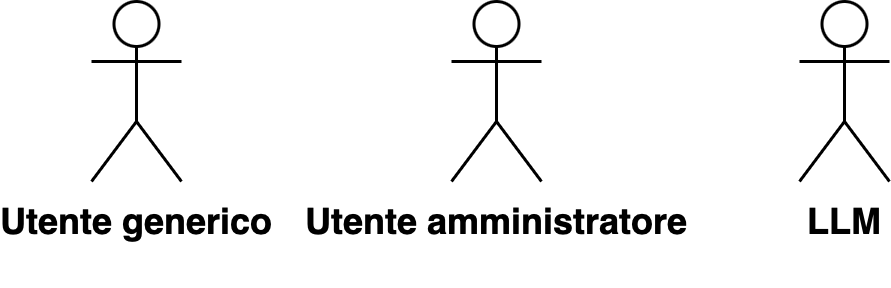
\includegraphics[width=0.6\textwidth]{actors.png}
    \caption{Attori dei casi d'uso}
    \label{fig:attori}
\end{figure}
\subsection{Casi d'uso}
I diagrammi dei casi d'uso permettono di descrivere le interazione tra gli attori e il sistema.  
La convezione che ho utilizzato per la stesura dei casi d'uso è stata la seguente:
\begin{center}
    \textbf{{UC[Numero]}: nome del caso d'uso}
\end{center}
a cui ho associato una descrizione, la lista degli attori coinvolti, le precondizioni e le postcondizioni affinche il caso d'uso possa avvenire.
Per riassumere i casi d'uso, sono presenti dei diagrammi UML per una rappresentazione grafica degli scenari.
Gli \textit{use case} qui di seguito riportati rappresentano i casi d'uso principali e non banali del progetto.
\subsubsection{Sistema di proposte di risoluzione Jira}
\subsubsection{UC0: Autenticazione nel \textit{workspace} Jira} 
\textbf{Attori principali}: Utente generico \\
\textbf{Precondizioni}: L'utente vuole accedere al \textit{workspace} Jira \\
\textbf{Descrizione}: All'accesso al \textit{workspace} Jira, viene aperta una schermata di \textit{login} per l'autenticazione dell'utente \\
\textbf{Postcondizioni}: L'utente è autenticato nel \textit{workspace} Jira \\
\begin{figure}[H]
    \centering
    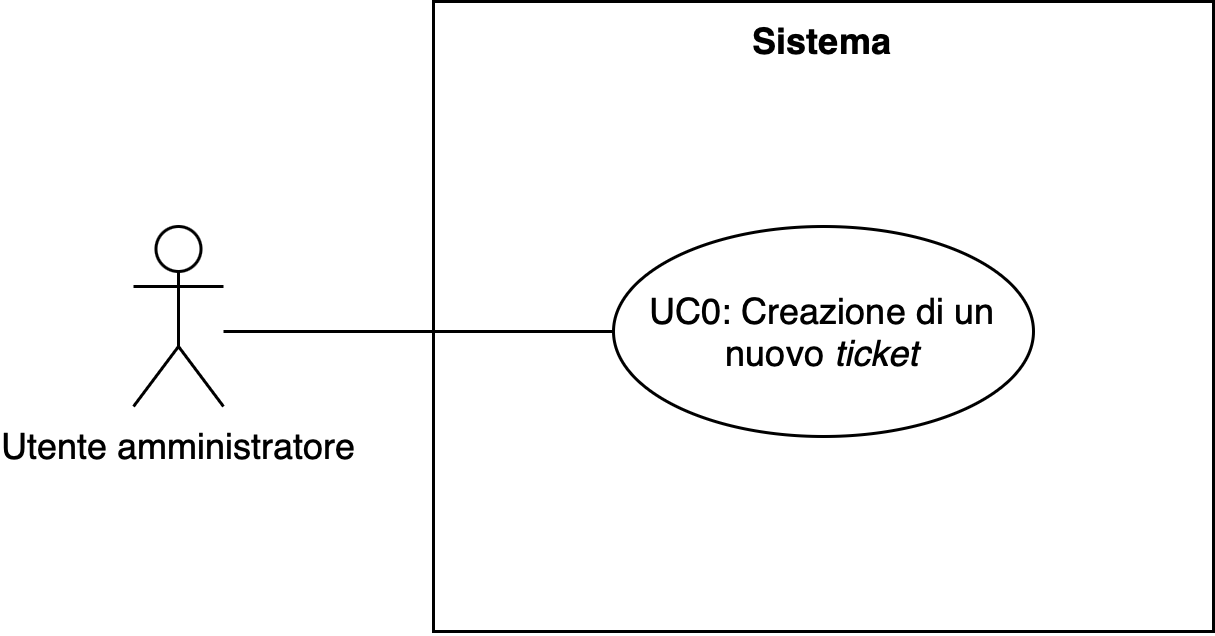
\includegraphics[width=0.63\textwidth]{uc0.png}
    \caption{Diagramma del caso d'uso UC0}
    \label{fig:UC0}
\end{figure}
\subsubsection{UC1: Creazione di un nuovo ticket}
\textbf{Attori principali}: Utente amministratore \\
\textbf{Precondizioni}: L'utente amministratore è autenticato nel \textit{workspace} Jira\\
\textbf{Descrizione}: L'utente amministratore crea un nuovo \textit{ticket} all'interno del progetto Jira \\
\textbf{Postcondizioni}: Il \textit{ticket} è stato creato \\
\begin{figure}[H]
    \centering
    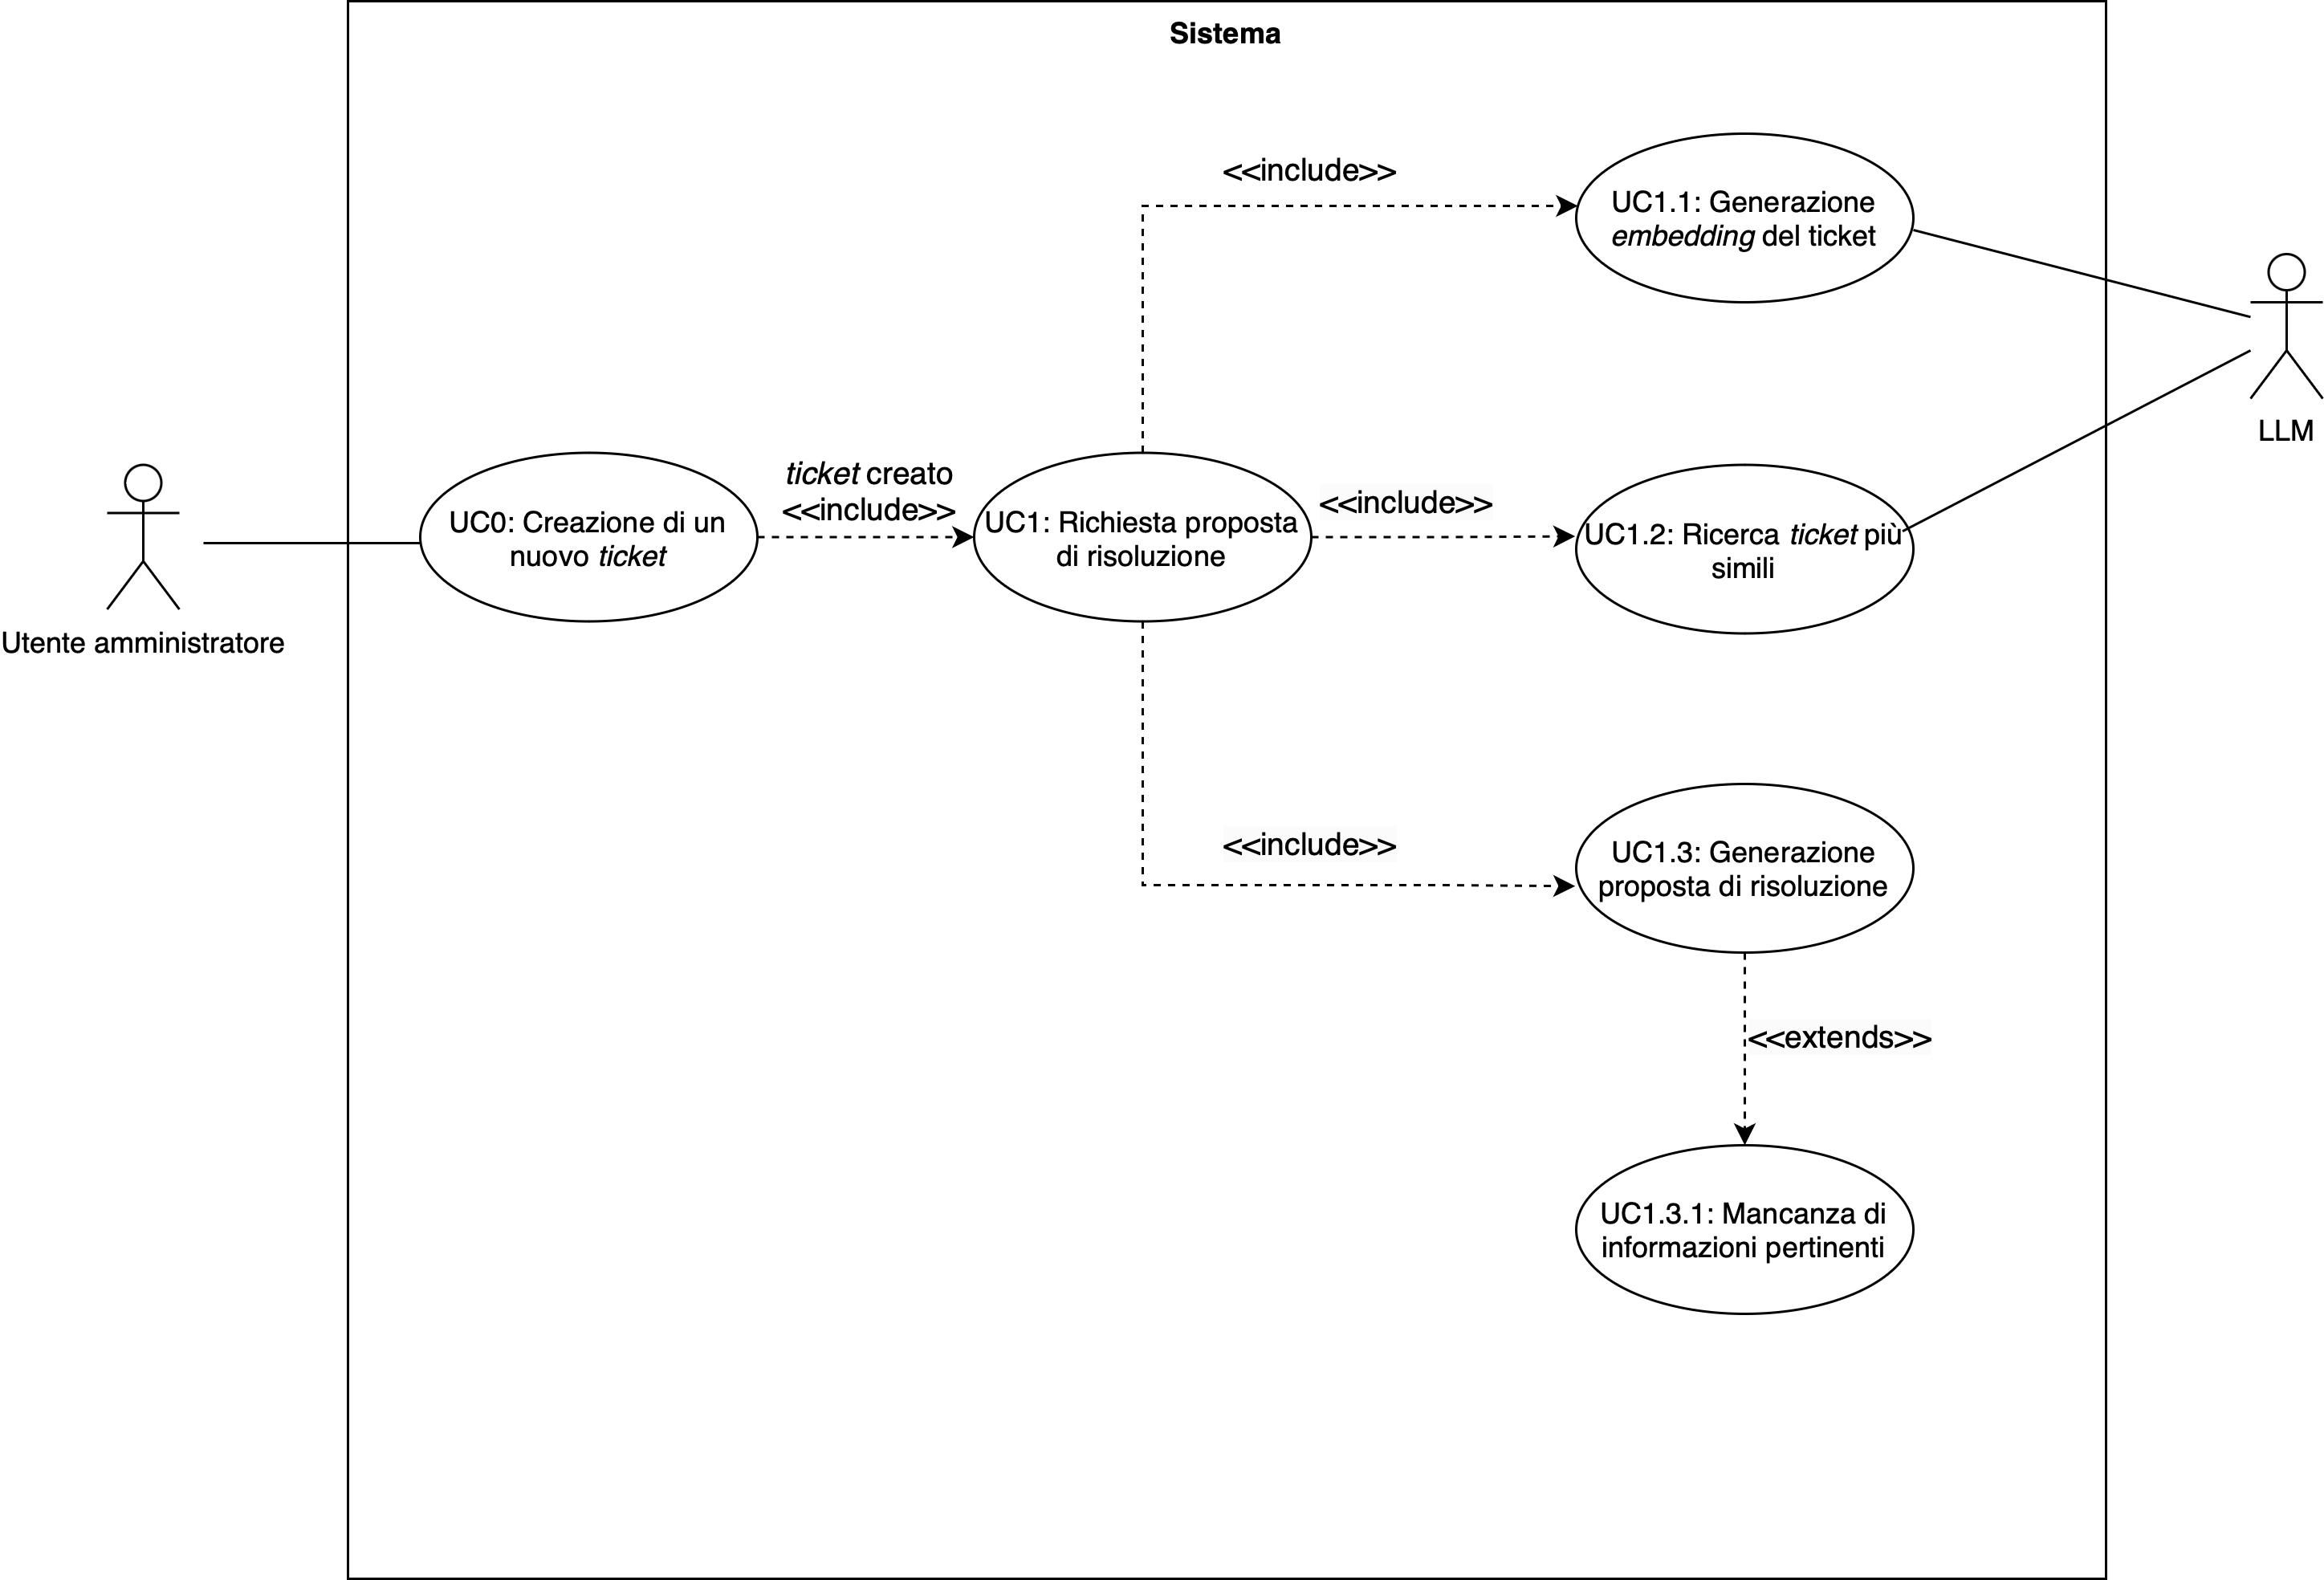
\includegraphics[width=0.63\textwidth]{uc1.png}
    \caption{Diagramma del caso d'uso UC0}
    \label{fig:UC1}
\end{figure}
\subsubsection{UC2: Richiesta proposta di risoluzione}
\textbf{Attori principali}: Utente amministratore \\
\textbf{Precondizioni}: L'utente amministratore ha creato un nuovo \textit{ticket} \\
\textbf{Descrizione}: Viene richiesto al sistema di generare una proposta di risoluzione per il \textit{ticket} appena creato \\
\textbf{Postcondizioni}: Il sistema inizia il processo di generazione della proposta di risoluzione \\

\subsubsection{UC2.1: Generazione \gls{embedding-g} del ticket}
\textbf{Attori principali}: \gls{llm} \\
\textbf{Precondizioni}: Il \textit{ticket} è stato creato ed è stata richiesta una proposta di risoluzione \\
\textbf{Descrizione}: Viene richiesto all'\gls{llm} di generare l'\gls{embedding-g} del \textit{ticket} per effettuare la ricerca dei \textit{ticket} completati più simili \\
\textbf{Postcondizioni}: L'\gls{embedding-g} del \textit{ticket} è stato generato \\

\subsubsection{UC2.2: Ricerca \textit{ticket} più simili}
\textbf{Attori principali}: Sistema \\ 
\textbf{Precondizioni}: È stato generato l'\gls{embedding-g} del \textit{ticket} creato\\
\textbf{Descrizione}: Il sistema effettua una ricerca vettoriale all'interno del \textit{database} con l'utilizzo dell'\gls{embedding-g}, per trovare i \textit{ticket} completati più simili al \textit{ticket} creato \\
\textbf{Postcondizioni}: I \textit{ticket} completati più simili vengono restuiti dal sistema \\

\subsubsection{UC2.3: Generazione proposta di risoluzione}
\textbf{Attori principali}: \gls{llm} \\
\textbf{Precondizioni}: Sono stati restituiti i \textit{ticket} completati più simili al \textit{ticket} creato \\
\textbf{Descrizione}: Viene richiesto all'\gls{llm} di generare una proposta di risoluzione per il \textit{ticket} creato usando come contesto i \textit{ticket} completati più simili \\
\textbf{Postcondizioni}: La proposta di risoluzione è stata generata ed inserita all'interno del campo adibito, del \textit{ticket} creato \\

\subsubsection{UC2.4: Mancanza di informazioni sufficienti}
\textbf{Attori principali}: \gls{llm} \\
\textbf{Precondizioni}: Non sono stati trovati \textit{ticket} completati simili al \textit{ticket} creato \\
\textbf{Descrizione}: Viene generata una risposta standard per informare l'utente amministratore che non sono stati trovati \textit{ticket} completati simili \\
\textbf{Postcondizioni}: Viene inserito un messaggio standard all'interno del campo adibito, del \textit{ticket} creato \\

\begin{figure}[H]
    \centering
    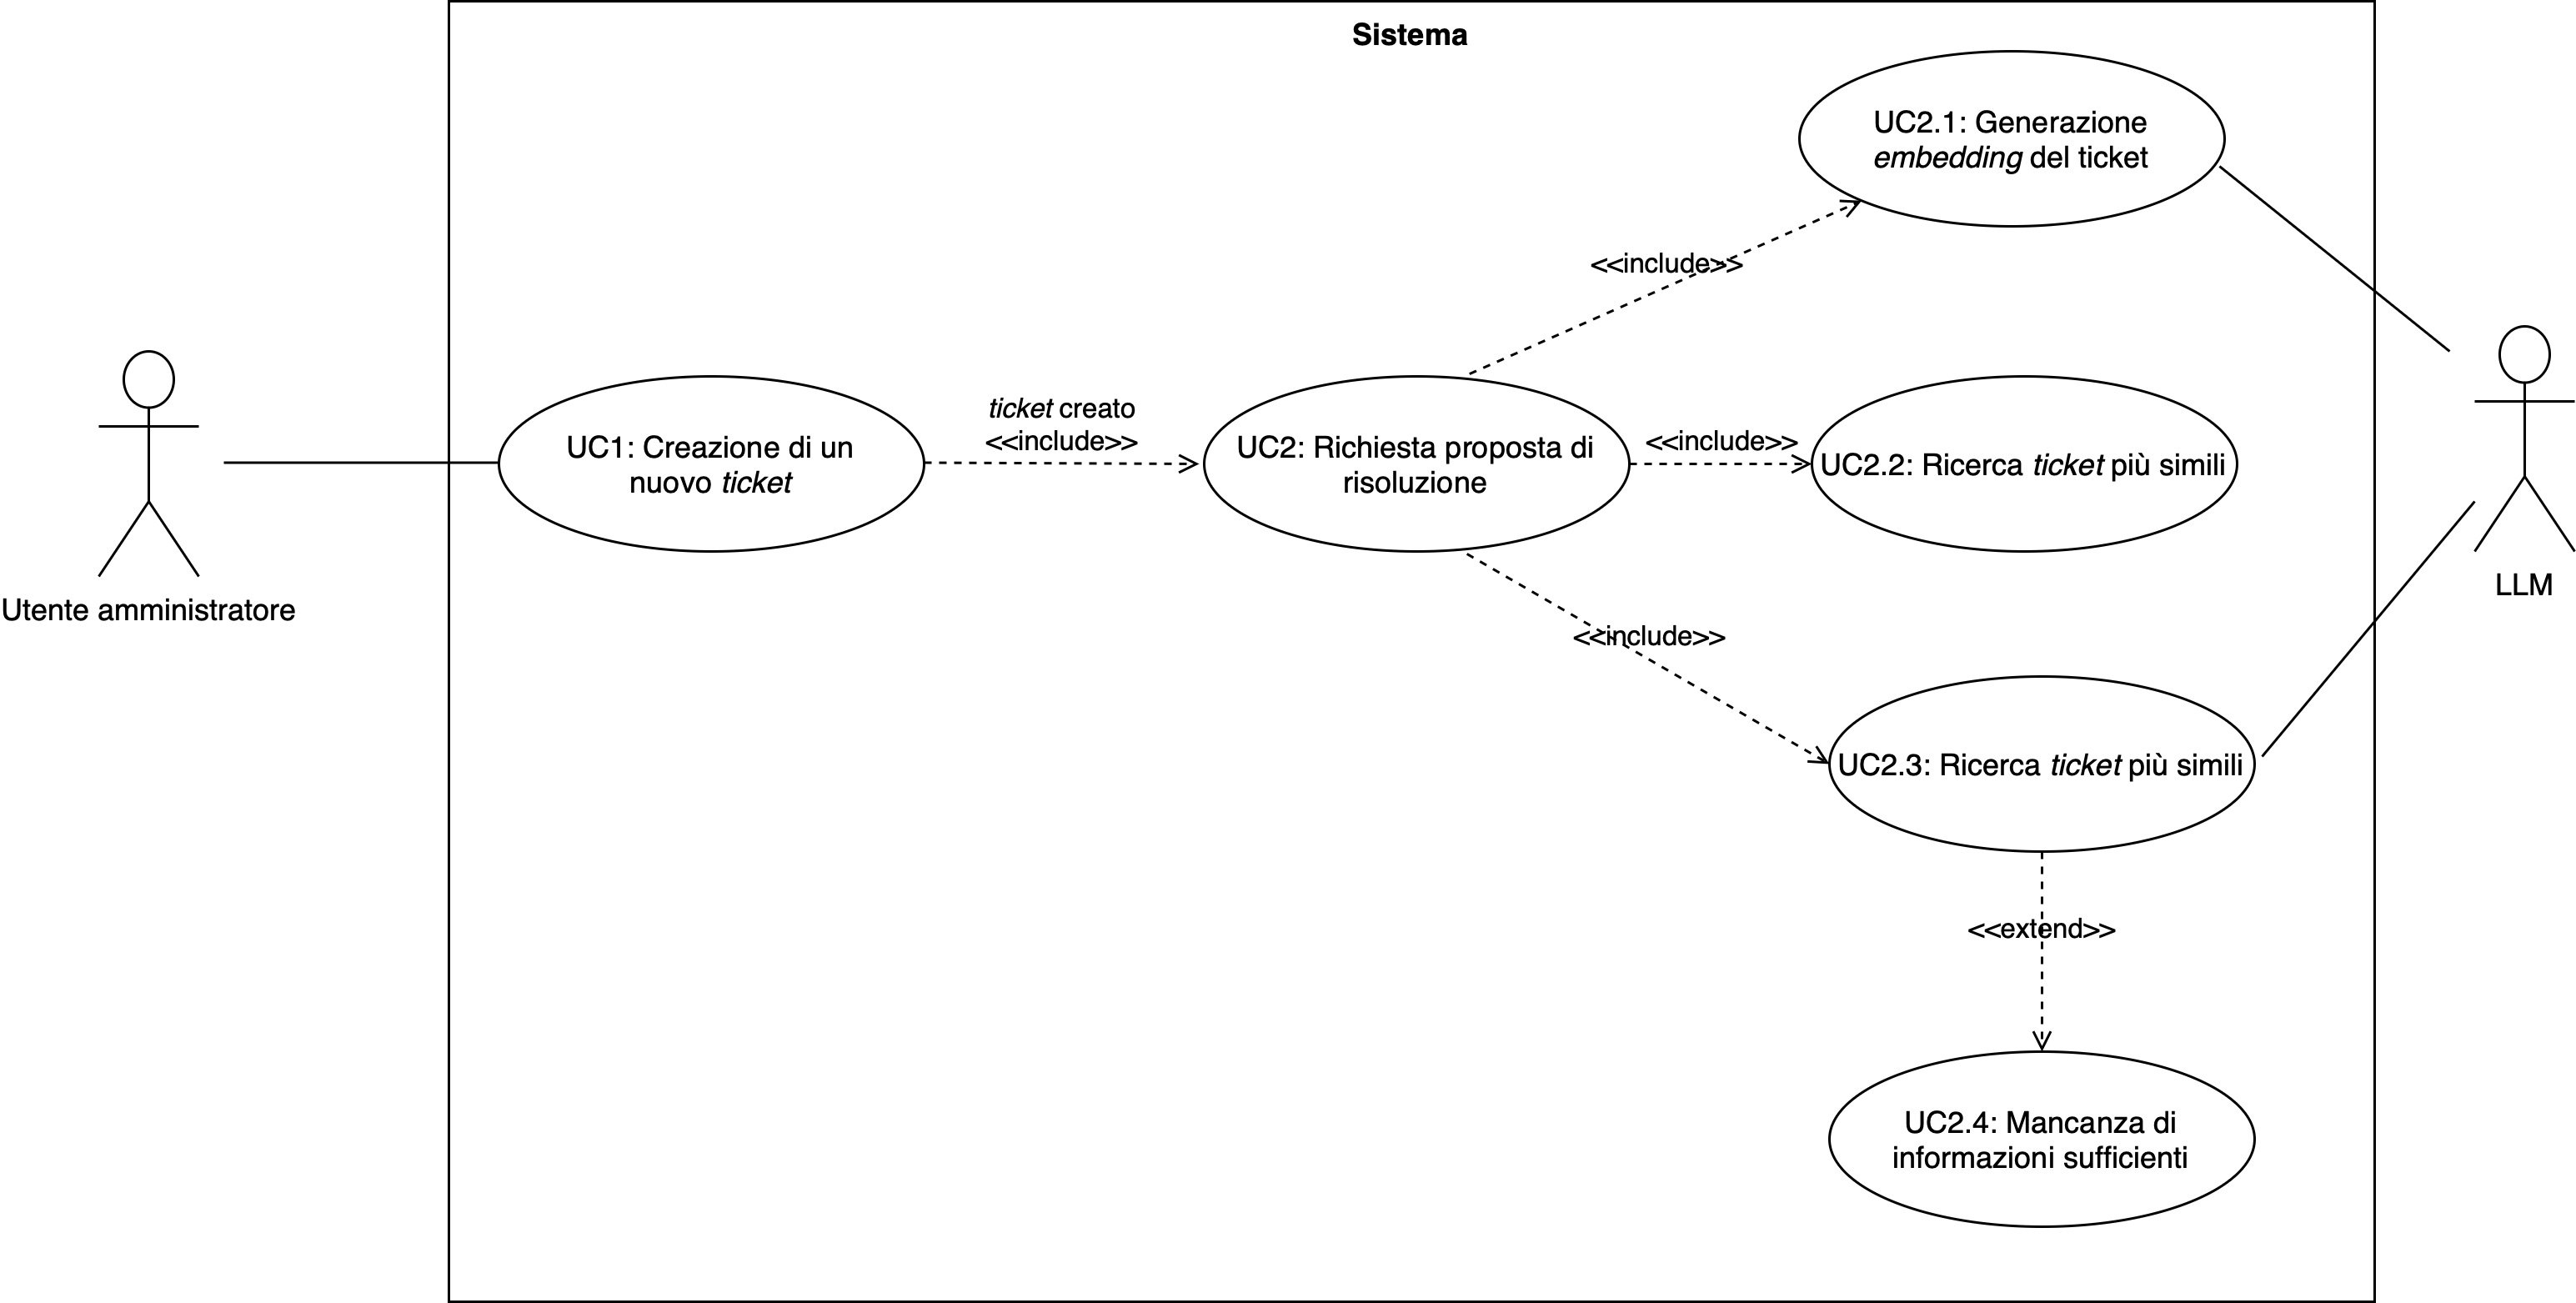
\includegraphics[width=0.9\textwidth]{uc2.png}
    \caption{Diagramma del caso d'uso UC2 e dei relativi sottocasi}
    \label{fig:UC2}
\end{figure}

\subsubsection{UC3: Chiusura di un \textit{ticket}}
\textbf{Attori principali}: Utente amministratore \\
\textbf{Precondizioni}: Il \textit{ticket} è stato completato \\
\textbf{Descrizione}: L'utente amministratore chiude il \textit{ticket} mettondolo in \textit{Done}\\ 
\textbf{Postcondizioni}: Il \textit{ticket} è stato chiuso \\

\begin{figure}[H]
    \centering
    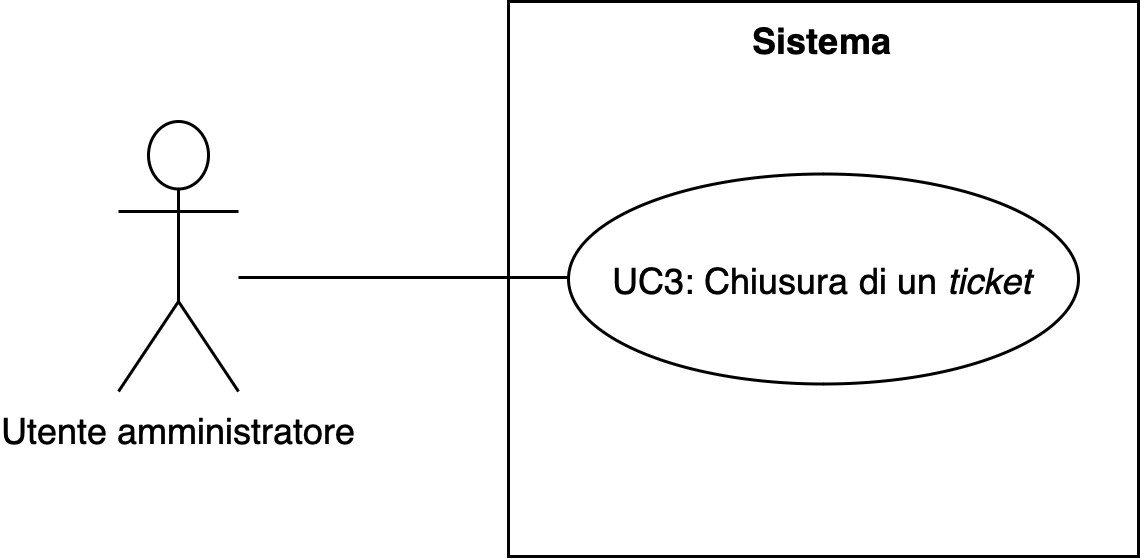
\includegraphics[width=0.6\textwidth]{uc3.png}
    \caption{Diagramma del caso d'uso UC3}
    \label{fig:UC3}
\end{figure}


\subsubsection{UC3.1: Generazione \gls{embedding-g} del \textit{ticket} completato}
\textbf{Attori principali}: \gls{llm} \\
\textbf{Precondizioni}: Il \textit{ticket} è stato chiuso \\
\textbf{Descrizione}: Viene richiesto all'\gls{llm} di generare l'\gls{embedding-g} del \textit{ticket} completato per poterlo poi salvare nel \textit{database} MongoDB \\
\textbf{Postcondizioni}: L'\gls{embedding-g} del \textit{ticket} è stato generato \\

\subsubsection{UC4: Salvataggio \textit{ticket} su \textit{database} MongoDB}
\textbf{Attori principali}: Sistema \\
\textbf{Precondizioni}: Il \textit{ticket} è stato compleato e in stato \textit{Done} \\
\textbf{Descrizione}: Il \textit{ticket} viene salvato su \textit{database} MongoDB con il suo relativo \textit{embedding} \\
\textbf{Postcondizioni}: Il \textit{ticket} è stato salvato su \textit{database} MongoDB con il suo relativo \textit{embedding} \\
\begin{figure}[H]
    \centering
    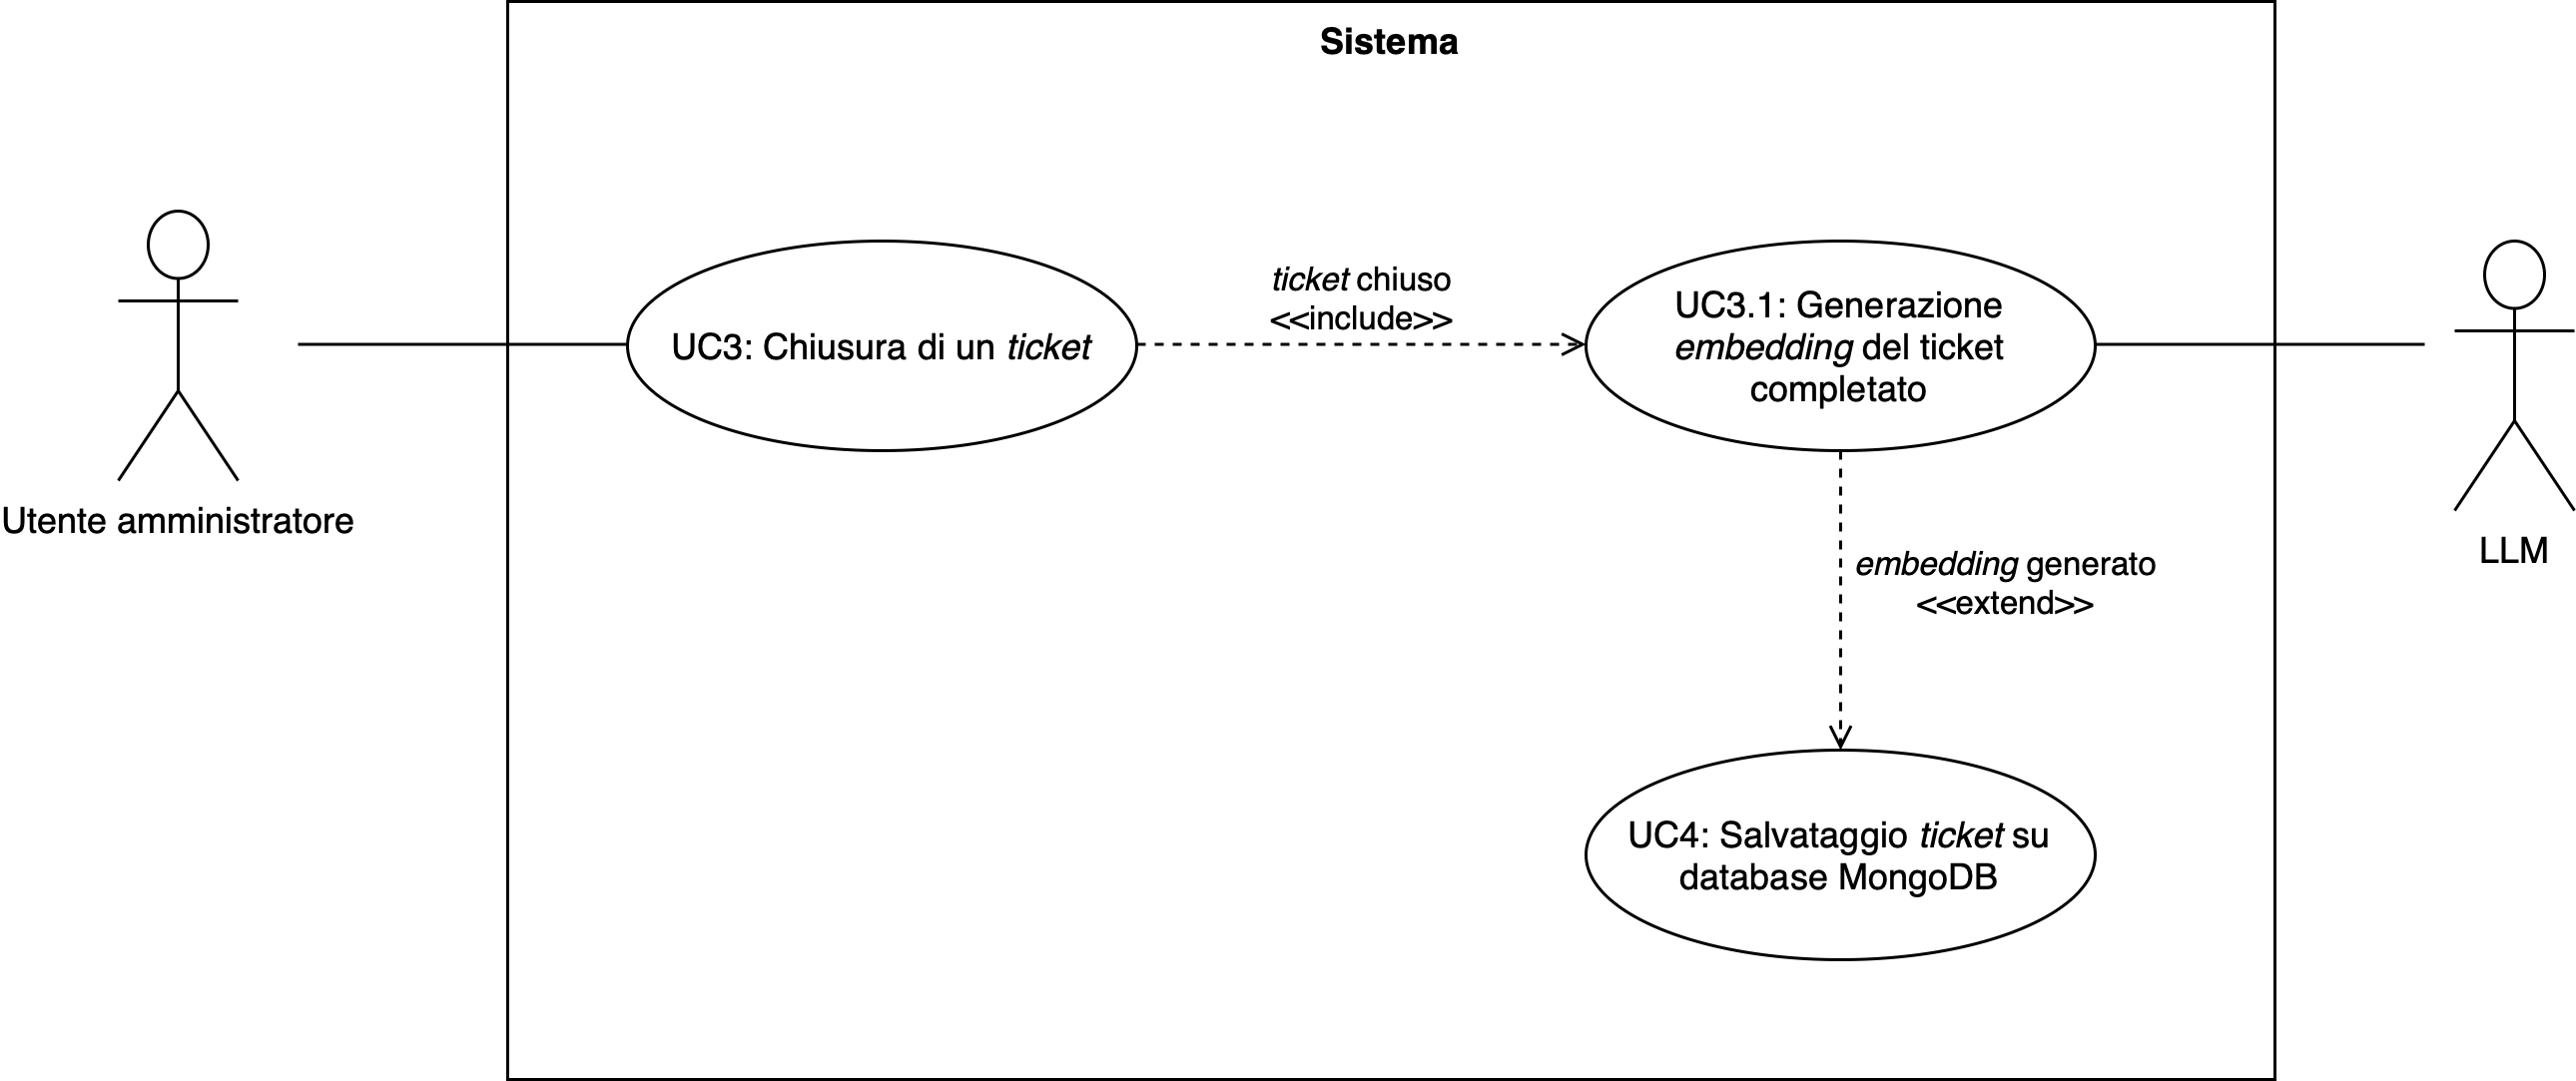
\includegraphics[width=0.75\textwidth]{uc4.png}
    \caption{Diagramma del caso d'uso UC5}
    \label{fig:UC5}
\end{figure}

\subsubsection{\textit{Chatbot}}

\subsubsection{UC0: Autenticazione nel \textit{chatbot}}
\textbf{Attori principali}: Utente generico \\
\textbf{Precondizioni}: L'utente vuole accedere al \textit{chatbot} \\
\textbf{Descrizione}: All'accesso al \textit{chatbot}, viene aperta una schermata di \textit{login} per l'autenticazione dell'utente \\
\textbf{Postcondizioni}: L'utente è autenticato nel \textit{chatbot} \\
\begin{figure}[H]
    \centering
    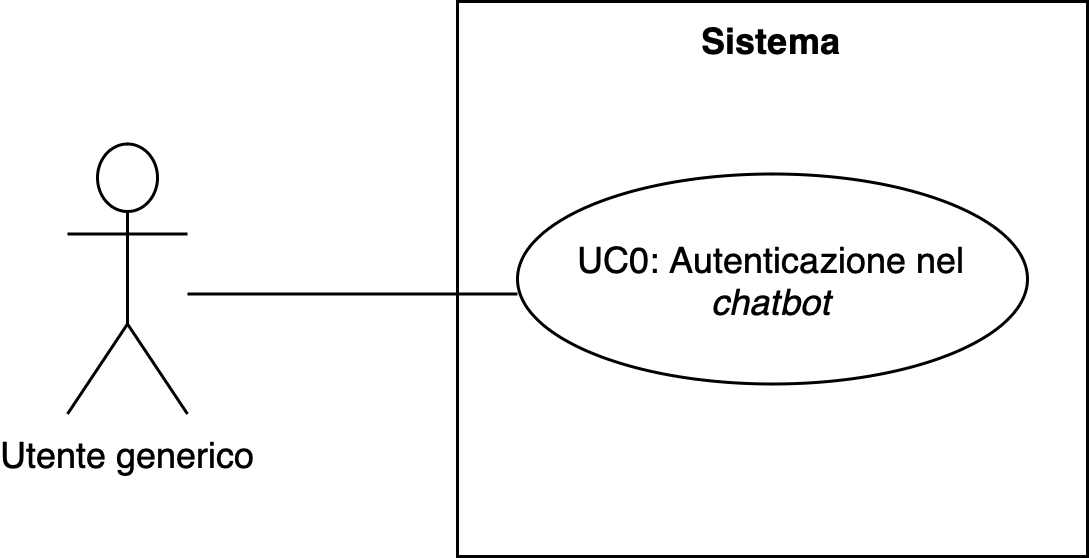
\includegraphics[width=0.45\textwidth]{uc0Chatbot.png}
    \caption{Diagramma del caso d'uso UC0 - \textit{Chatbot}}
    \label{fig:UC0Chatbot}
\end{figure}

\subsubsection{UC1: Autenticazione per il \textit{database} MongoDB}
\textbf{Attori principali}: Utente amministratore \\
\textbf{Precondizioni}: L'utente amministratore è autenticato nel \textit{chatbot} \\
\textbf{Descrizione}: L'utente amministratore si autentica per poter accedere al \textit{database} MongoDB e poter ricercare i \textit{ticket} più simili \\
\textbf{Postcondizioni}: L'utente amministratore è autenticato per il \textit{database} MongoDB \\
\begin{figure}[H]
    \centering
    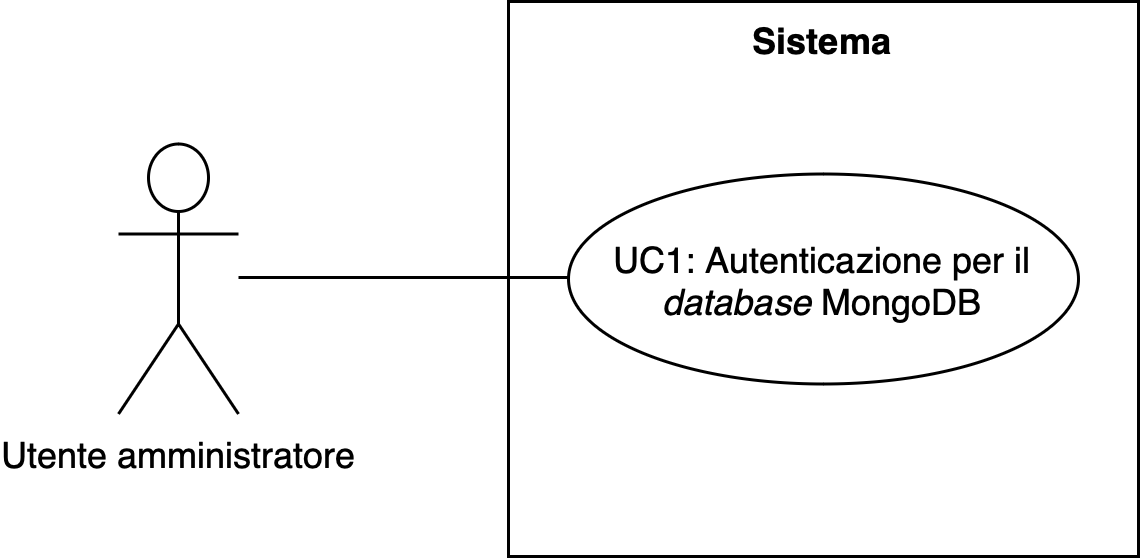
\includegraphics[width=0.6\textwidth]{uc1Chatbot.png}
    \caption{Diagramma del caso d'uso UC1 - \textit{Chatbot}}
    \label{fig:UC1Chatbot}
\end{figure}


\subsubsection{UC2: Scelta del modello \gls{llm}}
\textbf{Attori principali}: Utente amministratore \\
\textbf{Precondizioni}: L'utente amministratore è autenticato nel \textit{chatbot} \\
\textbf{Descrizione}: L'utente amministratore sceglie il modello \gls{llm} con cui interrogare il \textit{chatbot} \\
\textbf{Postcondizioni}: Il modello \gls{llm} è stato scelto \\
\begin{figure}[H]
    \centering
    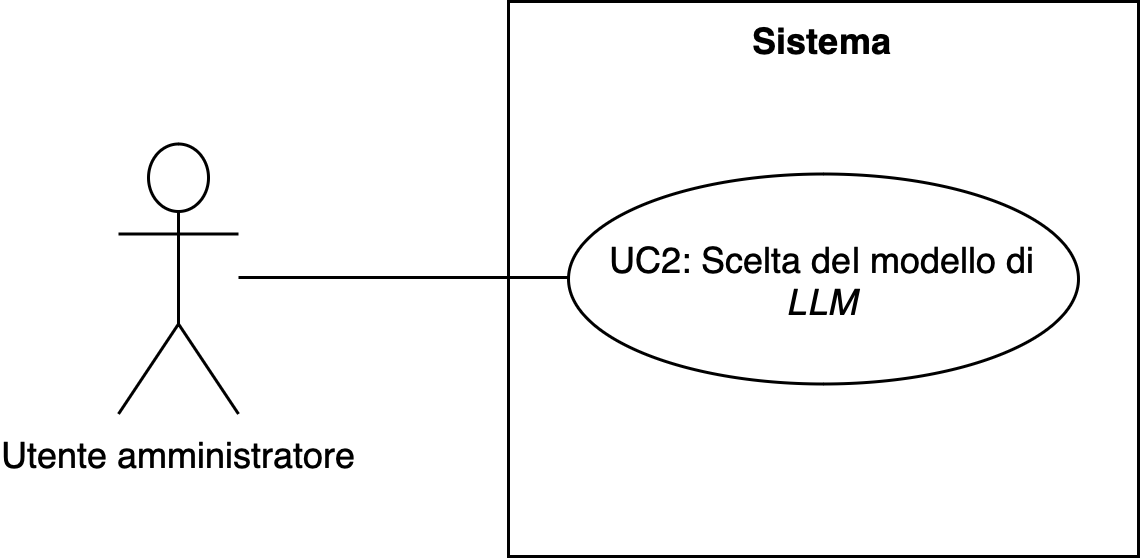
\includegraphics[width=0.6\textwidth]{uc2Chatbot.png}
    \caption{Diagramma del caso d'uso UC2 - \textit{Chatbot}}
    \label{fig:UC2Chatbot}
\end{figure}


\subsubsection{UC3: Inserimento del testo di un \textit{ticket} all'interno della \textit{chat} del \textit{chatbot}}
\textbf{Attori principali}: Utente amministratore \\
\textbf{Precondizioni}: L'utente amministratore ha scelto il modello \gls{llm} con cui interrogare il \textit{chatbot} \\
\textbf{Descrizione}: L'utente amministratore interroga il \textit{chatbot} sui \textit{ticket} Jira \\
\textbf{Postcondizioni}: Il \textit{chatbot} richiede la richiesta di proposta di risoluzione al sistema \\

\subsubsection{UC3.1: Generazione \gls{embedding-g} del testo inserito dall'utente}
\textbf{Attori principali}: \gls{llm} \\
\textbf{Precondizioni}: L'utente amministratore ha inserito il testo del \textit{ticket} per interrogare il \textit{chatbot} \\
\textbf{Descrizione}: Viene generato l'\gls{embedding-g} del testo inserito dall'utente per effettuare la ricerca dei \textit{ticket} completati più simili \\

\subsubsection{U3.2: Ricerca \textit{ticket} più simili all'interno del \textit{database} MongoDB}
\textbf{Attori principali}: Sistema \\
\textbf{Precondizioni}: È stato generato l'\gls{embedding-g} del testo inserito dall'utente \\
\textbf{Descrizione}: Il sistema effettua una ricerca vettoriale all'interno del \textit{database} con l'utilizzo dell'\gls{embedding-g}, per trovare i \textit{ticket} completati più simili al testo inserito dall'utente \\
\textbf{Postcondizioni}: I \textit{ticket} completati più simili vengono restuiti dal sistema \\

\subsubsection{UC3.3: Generazione proposta di risoluzione}
\textbf{Attori principali}: \gls{llm} \\
\textbf{Precondizioni}: Sono stati restituiti i \textit{ticket} completati più simili al testo inserito dall'utente \\
\textbf{Descrizione}: Viene richiesto all'\gls{llm} di generare una proposta di risoluzione per il testo inserito dall'utente usando come contesto i \textit{ticket} completati più simili \\
\textbf{Postcondizioni}: La proposta di risoluzione è stata generata e restituita all'utente, nell'interfaccia del \textit{chatbot} \\


\begin{figure}[H]
    \centering
    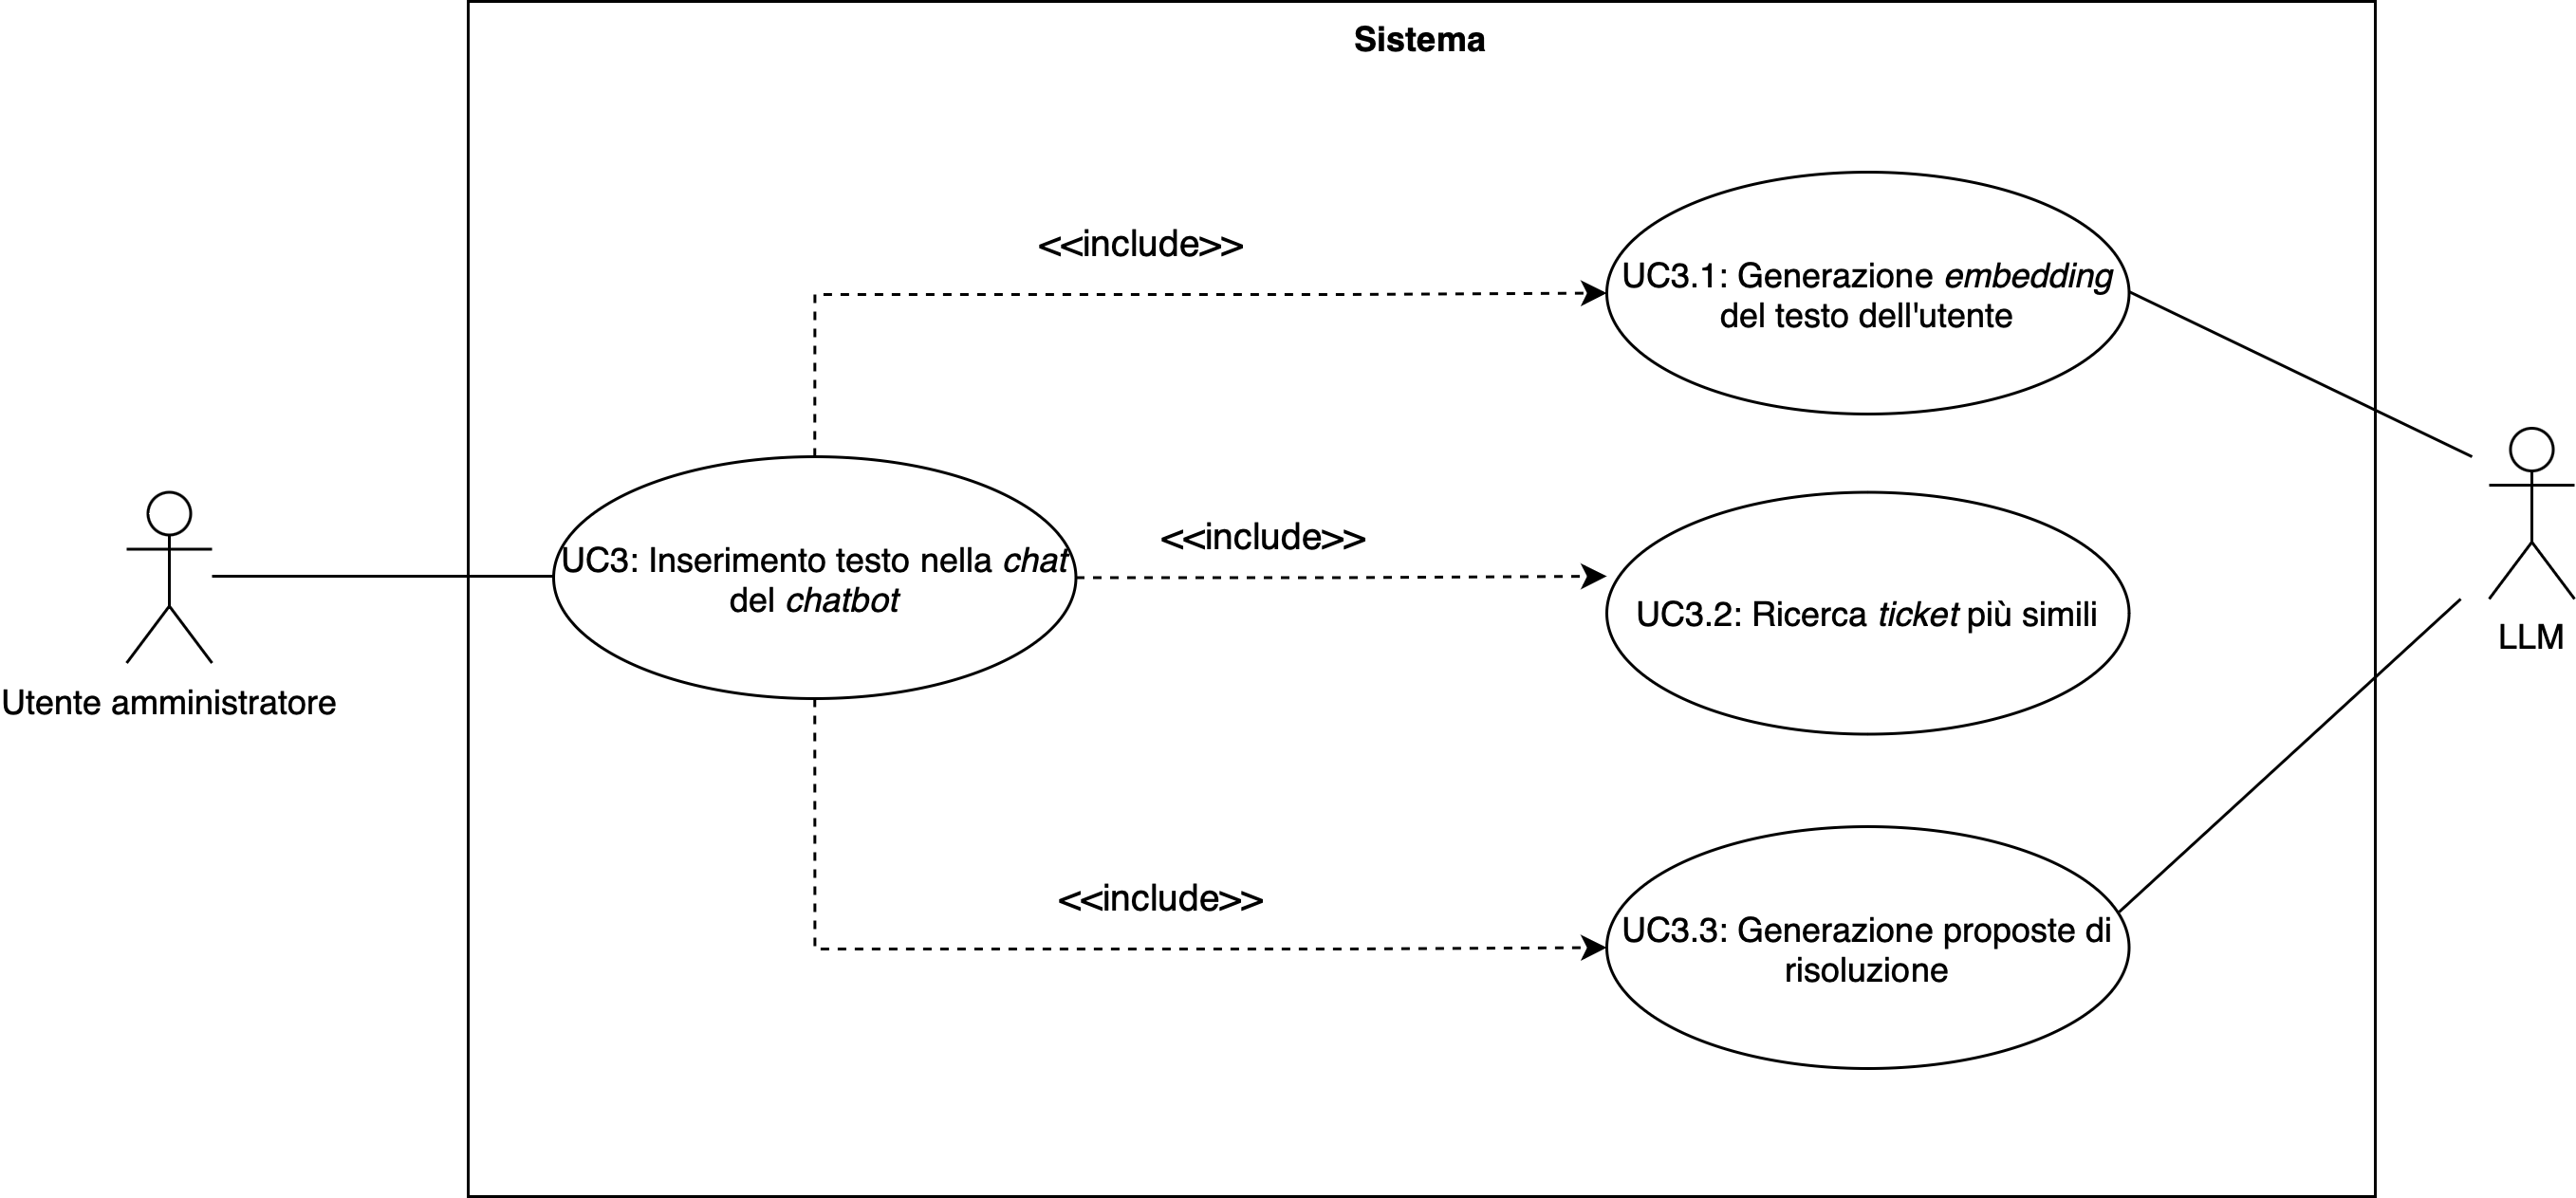
\includegraphics[width=0.9\textwidth]{uc3Chatbot.png}
    \caption{Diagramma del caso d'uso UC3 e dei relativi sottocasi}
    \label{fig:UC3Chatbot}
\end{figure}

\section{Progettazione}
\subsection{Architettura del sistema \textit{Jira}}
Descrizione dell'architettura ad eventi progettata per il sistema Jira
\subsection{Architettura del \textit{Chatbot}}
Descrizione dell'architettura del Chatbot tramite il framework Streamlit.
\section{Codifica}
Descrizione dell'attività di codifica delle componenti \textit{AWS Lambda} e del \textit{chatbot}
\section{Verifica e validazione}
Descrizione del processo di Verifica e validazione delle funzione lambda create, attraverso la creazione di eventi di test.
Per quanto riguarda il chatbot, verrà illustrato il perchè non saranno presenti metriche di test.

\section{Risultato finale}
Descrizione del risultato finale ottenuto, ad alto livello.